\documentclass[10pt]{article}
\usepackage[utf8]{inputenc}
\usepackage[spanish]{babel}
\usepackage[usenames,dvipsnames,svgnames,table]{xcolor}
\usepackage{multirow}
\usepackage{diagbox}
\usepackage{booktabs}
\usepackage{anysize} 
\usepackage{hyperref}
\usepackage{helvet}
\renewcommand\refname{Referencias}
\marginsize{2cm}{2cm}{2.0cm}{2cm}
\usepackage{enumitem}
\usepackage{setspace}
\usepackage{scrextend}
\usepackage{amssymb}
\usepackage{mathtools}
\addtokomafont{labelinglabel}{\sffamily}

%% Graphics
\usepackage{graphicx}
\usepackage{color}
\usepackage{gensymb}
\usepackage{multirow}
\usepackage{caption}
\usepackage{float}
\graphicspath{{img/}}
\setlength{\parindent}{0cm}


\hypersetup{
	colorlinks=true,
	linkcolor=blue,
	filecolor=magenta,
	urlcolor=cyan,
	citecolor=blue
}





\begin{document}
	
	\title{Fundamentos de Bases de Datos \\
		Practica 7\\ Normalización de la Base de Datos
	} 
	\author{}
	\date{16 de Abril del 2019}
	\maketitle
	

El objetivo en esta práctica es normalizar la base de datos de acuerdo al caso 
de uso que hemmos venido usando. Normalizar la base de datos evita almacenar 
información redundante,  para esta practica se usa la tercera formal normal (3NF).

\section{Esquema relacional no normalizado}

\begin{figure}[H]
	\centering
	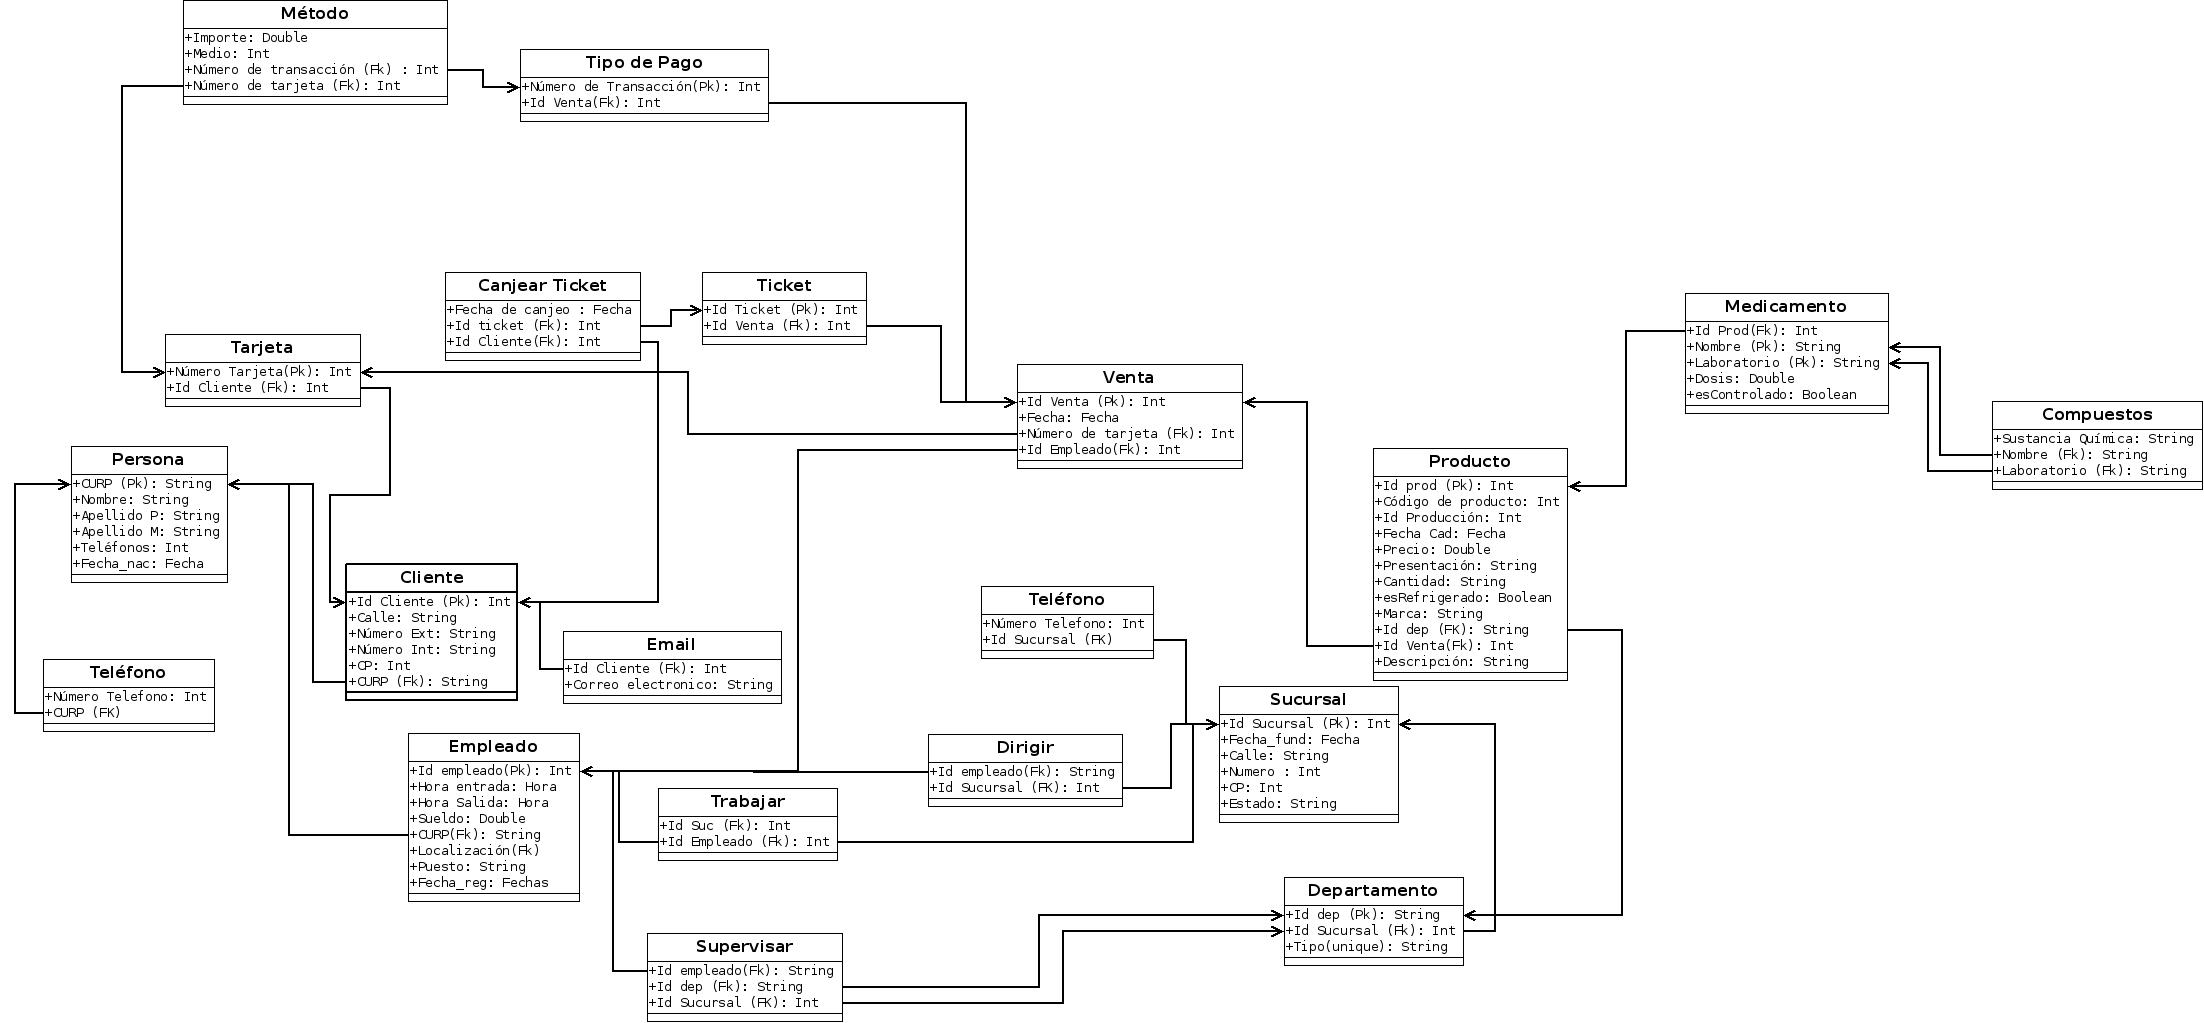
\includegraphics[scale=0.2 ]{practica05.jpeg}
	\caption{Esquema de la práctica anterior}
	\label{fg:esqA}
\end{figure}

\subsection{Cambios antes de la normalización}
\begin{itemize}
	\item Se trasforam la relación de Departamento a una relación de pertenencia
	entre una sucursal y un catálogo de tipos.
\end{itemize}

\begin{figure}[H]
	\centering
	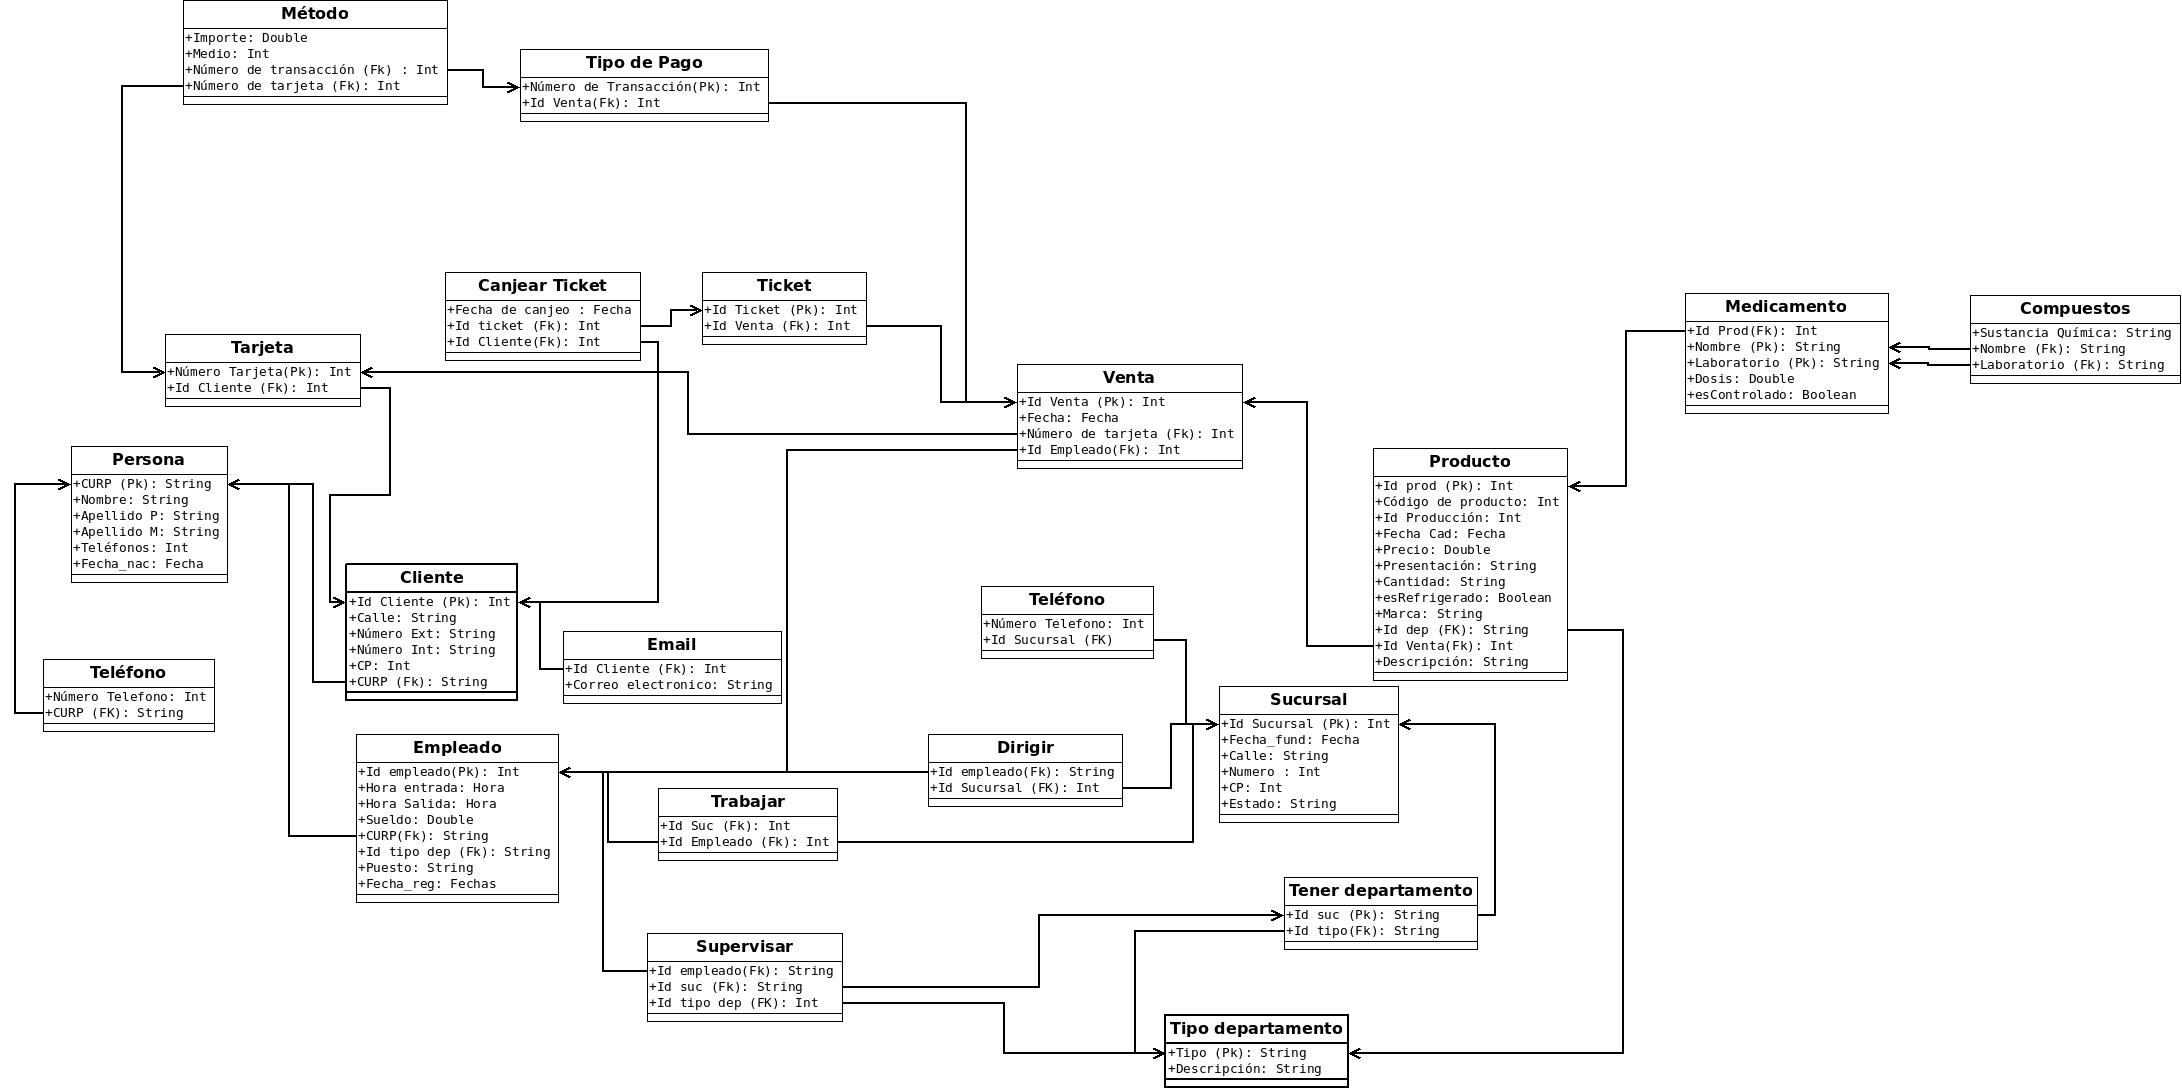
\includegraphics[scale=0.2 ]{practica07.jpeg}
	\caption{Esquema justo antes de la normalización}
	\label{fg:esNN}
\end{figure}

\section{Definiendo dependencias funcionales para el caso de uso}

\subsection{Tablas con dependencias únicamente triviales}
\begin{enumerate}
	\item Método\\
	Tanto el importe como el medio sólo son valores para representar la cantidad
	de dinero, que no son únicos entre transacciones.\\
	Una transacción puede tener varios métodos de pago, así que tampoco
	puede determinar nada.\\
	Y una tarjeta puede tener varias instancias de método de pago, por lo que
	tampoco puede identificar a nada. Además de que este campo puede ser nulo.\\
	Entonces las únicas dependencias funcionales de la relación son las
	triviales.\\
	Por lo que la relación ya está normalizada.
	\item Tipo de pago \\
	Una venta puede tener varias transacciones, por lo que el identificador de
	la venta no determina nada. El número de transacción, que es la llave, 
	determina a los demás.\\
	Entonces, las únicas dependencias funcionales son las triviales o la
	generada por la llave.\\
	Entonces la relación ya está normalizada.
	\item Tarjeta \\
	Un cliente puede tener varias tarjetas, así que el identificador de cliente 
	no puede determinar nada. \\
	El número de tarjeta, que es la llave, determina todo. \\
	Entonces las únicas dependencias funcionales que hay son las triviales o la
	inducida por la llave.\\
	Por lo que la relación ya está normalizada.
	\item Canjear Ticket \\
	La fecha no puede determinar nada. \\ 
	Un clienten canjea varios tickets, así que tampoco el cliente determina
	nada. Y se pueden canjear el mismo día, así que la fecha con el cliente
	tampoco determina nada extra.\\
	El identificador del ticket es único, pues un ticket solo se canjea una vez.
	Entonces el identificador del ticket determina a todo lo demás, por lo que
	es llave.\\
	Entonces las únicas dependencias funcionales que hay son las triviales o una
	inducida por una llave candidata.\\
	Por lo que la relación ya está normalizada.
	\item Ticket \\
	Una venta puede tener varios tickets (cuentas separadas) así que el
	identificador de la venta no determina nada.\\
	El identificador del ticket es la llave, y determina lo demás.\\
	Entonces las únicas dependecias funcionales son las triviales o las
	inducidas por la llave.\\
	Entonces la relación ya está normalizada.
	\item {Venta}
	Puede haber varias ventas por día, así que la fecha no determina nada extra.\\
	Una tarjeta puede usarse para varias ventas, así que el número de tarjeta no
	determna nada extra. Esas ventas pueden ser el mismo día, por lo que la fecha
	junto con el número de tarjeta no determina nada extra.\\
	Un empleado puede atender varias ventas así que el identificador de cliente
	no determina nada extra. También puede atender varias ventas el mismo día, y
	ventas diferentes que usaron la misma tarjeta así que el empledao junto con
	la fecha o la tarjeta no determinan nada extra.\\
	El identificador de venta es la llave, así que determina todo.\\
	Entonce en la relación sólo hay dependecias funcionales triviales o la
	inducida por la llave.\\
	Entonecs la relación ya está normalizada.
	\item Medicamento \\
	El laboratorio puede tener varios medicamentos, así queno determina nada
	extra. \\
	La dosis tampoco puede determinar nada extra, pues puede repetirse, al igual
	que la dosis con el laboratorio.\\
	Igualmente, la bandera sobre si es controlado no determina nada extra, así
	como tampoco esa bandera junto con el nombre del laboratorio o la dosis.\\
	El identificador del producto y el nombre del medicamento son la llave de la
	relación, por lo que determinan todo.\\
	Entonces en la relación las únicas dependencias funcionales son las
	triviales o las inducidas por la llave.\\
	Por lo que la relación ya está normalizada.
	\item Compuestos \\
	El nombre del compuesto es el determinante, que se debe juntar con las
	llaves foráneas.\\
	Entonces  todos los atributos son la llave.\\
	Por lo que sólo hay dependencias funcionales triviales y la relación ya está
	normalizada.
	\item Teléfono Sucursal
	El número es un determinante, por lo que es una llave.\\
	Una sucursal puede tener varios teléfonos, así que la sucursal no determina
	nada extra.\\
	Entonces todas las dependencias funcionales son triviales o la inducida por
	la llave.\\
	Por lo que la relación ya está normalizada.
	\item Teléfono Persona
	El número es un determinante, por lo que es una llave.\\
	Un cliente puede tener varios teléfonos, así que el identificador de cliente
	no determina nada extra.\\
	Entonces todas las dependencias funcionales son triviales o la inducida por
	la llave.\\
	Por lo que la relación ya está normalizada.
	\item Email
	El correo es un determinante, pues dos clientes no puede tener el mismo
	correo, por lo que es una llave.\\
	Un cliente puede tener varios correo, así que la sucursal no determina
	nada extra.\\
	Entonces todas las dependencias funcionales son triviales o la inducida por
	la llave.\\
	Por lo que la relación ya está normalizada.
	\item Trabajar
	Un empleado puede trabajar en varias sucursales y una sucursal puede tener
	varios trabajadores. \\
	Entonces todas las dependencias funcionales son triviales, por lo que la
	relación ya está normalizada.
	\item Dirigir \\
	Un empleado puede dirigir varias sucursales, por lo que no determina nada
	extra.\\
	Una sucursal sólo tiene un gerente, así que es única. Entonces puede ser
	llave.\\
	Entonces todas las dependencias funcionales son triviales o son las
	inducidas por la llave.\\
	Por lo que la relación ya está normalizada.
	\item Supervisar
	Un empleado puede supervisar varios departamentos, por lo que no determina nada
	extra.\\
	Un departamento sólo tiene un supervisor, así que es único. Entonces puede ser
	llave.\\
	Entonces todas las dependencias funcionales son triviales o son las
	inducidas por la llave.\\
	Por lo que la relación ya está normalizada.
	\item Tener departamento
	Una sucursal tiene varios departamentos, así que no puede determinar nada
	extra.\\
	Un tipo de departamentos puede estar en varias sucursales, así que tampoco
	determina nada extra.\\
	Entonces todas las dependencias funcionales son triviales.\\
	Entonces la relación ya está normalizada.
	\item Tipo Departamento
	La descripción podríano ser única, por lo que eno determina nada extra.\\
	El identificador también es llave y determina a lo demás.\\
	Entonces las dependencias funcionales son las generadas por llaves. \\
	Por lo que la relación ya está normalizada.
\end{enumerate}

\subsection{Relacion Empleado}
\subsection{Relacion Cliente}
\subsection{Relacion Persona}

\subsection{Relacion Producto}

%\noindent \textbf{PRODUCTO}\textit{(Id\_Producto, Código\_Barras, Id\_Producción, %Fecha\_Cad, Precio, Presentación, Cantidad, esRefrigerado, Marca, Id\_Departamento, %Id\_Venta, Descripción)}\\



Para facilitar la definición de las dependencias funcionales de la relación Producto nos conviene etiquetarla de la siguiente manera:

\begin{align*}
\overbrace{ \textbf{PRODUCTO}}^{\textbf{{P}}}&(\overbrace{ Id\_Producto}^{\textbf{\textcolor{RoyalBlue}{A}}},\,\overbrace{Codigo\_Barras}^{\textbf{\textcolor{RoyalBlue}{B}}},\,\overbrace{Id\_Produccion}^{\textbf{\textcolor{RoyalBlue}{C}}},\,\overbrace{Fecha\_Cad}^{\textbf{\textcolor{RoyalBlue}{D}}},\,\overbrace{Precio}^{\textbf{\textcolor{RoyalBlue}{E}}},\,\overbrace{Presentacion}^{\textbf{\textcolor{RoyalBlue}{F}}},\\&\overbrace{Cantidad}^{\textbf{\textcolor{RoyalBlue}{G}}},\,\overbrace{esRefrigerado}^{\textbf{\textcolor{RoyalBlue}{H}}},\,\overbrace{Marca}^{\textbf{\textcolor{RoyalBlue}{I}}},\,\overbrace{Id\_Departamento}^{\textbf{\textcolor{RoyalBlue}{J}}},\,\overbrace{Id\_Venta}^{\textbf{\textcolor{RoyalBlue}{K}}},\,\overbrace{Descripcion}^{\textbf{\textcolor{RoyalBlue}{L}}})\\
&= \textbf{P}(\mathrm{A,B,C,D,E,F,G,H,I,J,K,L})
\end{align*}

%\overbrace{,}^{\textbf{\textcolor{Blue}{}}}
Las siguientes dependencias funcionales para esta relacion son:\\

$$\mathcal{F}=\mathrm{\{ BIFG \rightarrow E, BC \rightarrow D, B \rightarrow FGHI \}}$$

Para normalizar primero tenemos que calcular la cerradura para cada dependencia funcional en $\mathcal{F}$,\\


$\mathrm{\{\textcolor{RoyalBlue}{BIFG}\}+= \{\textcolor{RoyalBlue}{BIFG}EH\}}$\\

$\mathrm{\{\textcolor{RoyalBlue}{BC}\}+= \{\textcolor{RoyalBlue}{BC}FGHIDE\}}$\\

$\mathrm{\{\textcolor{RoyalBlue}{B}\}+= \{\textcolor{RoyalBlue}{B}FGHIE\}}$\\


Observamos que a la cerradura de BC es que contiene el mayor numero de atributos y unicamente le faltan algunos atributos, por lo tanto una llave para \textbf{P} es \underline{ABCJKL} \\

Lo siguiente es buscar violaciones a la tercera forma normal, para eso hay que ver que no aparezca la llave en las dependecias funcionales, observamos que las tres dependencias son violaciones a la 3NF, así que se toma una dependencia funcional con mas de un atributo a la izquierda para ver si alguno de los atributos es superfluo.\\

\subsubsection{Superfluos a la Izquierda}
\noindent Tomamos $\mathrm{BIFG \rightarrow E}$, luego verificamos si algun atributo a la izquierda es superfluo. \\
\begin{itemize}


\item ¿B es superfluo? $\mathrm{IFG \rightarrow E}$\\

$\mathrm{\{\textcolor{RoyalBlue}{IFG}\}+= \{\textcolor{RoyalBlue}{IFG}\}}$\\
 	
Como E no aparece en la cerradura de IFG, por lo tanto se concluye que B no es superfluo.\\

\item ¿I es superfluo? $\mathrm{BFG \rightarrow E}$\\

$\mathrm{\{\textcolor{RoyalBlue}{BFG}\}+= \{\textcolor{RoyalBlue}{BFG}HIE\}}$\\

E aparece en la cerradura de BFG, por lo tanto se concluye que I es superfluo.\\

\item ¿F es superfluo? $\mathrm{BIG \rightarrow E}$\\

$\mathrm{\{\textcolor{RoyalBlue}{BIG}\}+= \{\textcolor{RoyalBlue}{BIG}FHE\}}$\\

E aparece en la cerradura de BIG, por lo tanto se concluye que F es superfluo.\\

\item ¿G es superfluo? $\mathrm{BIF \rightarrow E}$\\

$\mathrm{\{\textcolor{RoyalBlue}{BIF}\}+= \{\textcolor{RoyalBlue}{BIF}GHE\}}$\\

E aparece en la cerradura de BIF, por lo tanto se concluye que G es superfluo.\\

\end{itemize}

\noindent Como resultado de buscar superfluos por la izquierda obtenemos una $\mathcal{F}$ nueva,\\

$$\mathcal{F}=\mathrm{\{ B \rightarrow E, BC \rightarrow D, B \rightarrow FGHI \}}$$ \\ 
y por la regla de la union obtenemos $$\mathcal{F}=\mathrm{\{ BC \rightarrow D, B \rightarrow FGHIE \}}$$ \\

\subsubsection{Superfluos por la derecha}

Tenemos a $\mathrm{B \rightarrow FGHIE}$ y buscamos elementos superfluos a la derecha.\\

\begin{itemize}
	\item ¿F es superfluo? $\mathrm{B \rightarrow GHIE}$ \\
	$$\mathcal{F}'=\mathrm{\{ BC \rightarrow D, B \rightarrow GHIE \}}$$\\
	Calculamos la cerradura de B usando a $\mathcal{F}'$\\
	$\mathrm{\{\textcolor{RoyalBlue}{B}\}+= \{\textcolor{RoyalBlue}{B}GHIE\}}$\\
	
	F no aparece en la cerradura de B, por lo tanto F no es superfluo.
	
	\item ¿G es superfluo? $\mathrm{B \rightarrow FHIE}$ \\
	$$\mathcal{F}'=\mathrm{\{ BC \rightarrow D, B \rightarrow FHIE \}}$$\\
	Calculamos la cerradura de B usando a $\mathcal{F}'$\\
	$\mathrm{\{\textcolor{RoyalBlue}{B}\}+= \{\textcolor{RoyalBlue}{B}FHIE\}}$\\
	
	G no aparece en la cerradura de B, por lo tanto G no es superfluo.
	
	\item ¿H es superfluo? $\mathrm{B \rightarrow FGIE}$ \\
	$$\mathcal{F}'=\mathrm{\{ BC \rightarrow D, B \rightarrow FGIE \}}$$\\
	Calculamos la cerradura de B usando a $\mathcal{F}'$\\
	$\mathrm{\{\textcolor{RoyalBlue}{B}\}+= \{\textcolor{RoyalBlue}{B}FGIE\}}$\\
	
	H no aparece en la cerradura de B, por lo tanto H no es superfluo.
	
	\item ¿I es superfluo? $\mathrm{B \rightarrow FGHE}$ \\
	$$\mathcal{F}'=\mathrm{\{ BC \rightarrow D, B \rightarrow FGHE \}}$$\\
	Calculamos la cerradura de B usando a $\mathcal{F}'$\\
	$\mathrm{\{\textcolor{RoyalBlue}{B}\}+= \{\textcolor{RoyalBlue}{B}FGHE\}}$\\
	
	I no aparece en la cerradura de B, por lo tanto I no es superfluo.
	
	\item ¿E es superfluo? $\mathrm{B \rightarrow FGHI}$ \\
	$$\mathcal{F}'=\mathrm{\{ BC \rightarrow D, B \rightarrow FGHI \}}$$\\
	Calculamos la cerradura de B usando a $\mathcal{F}'$\\
	$\mathrm{\{\textcolor{RoyalBlue}{B}\}+= \{\textcolor{RoyalBlue}{B}FGHI\}}$\\
	
	E no aparece en la cerradura de B, por lo tanto E no es superfluo.\\
	
\end{itemize}	
	Así que la $\mathcal{F}_{min}$ es,\\
	
	$$\mathcal{F}'_{min}= \mathrm{\{ BC \rightarrow D, B \rightarrow FGHIE \}}$$
	
	Esto quiere decir que las relaciones quedan como: \\
	
	$\mathrm{R_1(B,C,D)}\,\,\, con \,\,\, \mathrm{ BC \rightarrow D}$\\
	$\mathrm{R_2(B,F, G, H, I, E)}\,\,\, con \,\,\, \mathrm{ B \rightarrow FGHIE}$\\
	
	El siguiente paso es verificar si la llave esta en alguna relaciones obtenidas, como la llave no aparece en ninguna relación la solución es agregar otra relación que la contenga.\\
	
	
	$\mathrm{R_3(A,B,C,J,K,L)}\,\,\, con \,\,\, \mathrm{ ABCJKL \rightarrow ABCJKL}$\\


   $\therefore \,\, \mathrm{R_1, R_2, R_3} $  es la normalización en 3NF para la relación Producto. 

   \subsection{Relacion Sucursal}
   La relación es 
   \[\overbrace{{\textbf{Sucursal}}}^{\textbf{S}} 
   (
	   \overbrace{Id\_Suc}^{I}, \overbrace{Fecha\_Fund}^{F},
	   \overbrace{Calle}^{C}, \overbrace{Numero}^{N}, Cp,
	   \overbrace{Estado}^{E}
	)
	= 
	\textbf{S}(I, F, C, N, Cp, E)
	\]
   Con las siguientes dependencias funcionales
   \[\mathcal{F} = \{I \rightarrow FCNCpE, Cp \rightarrow E\}\]
   Si bien existen dependencias funcionales que violan la tercera forma normal,
   sólo es una dependencia funcional que sólo concierne a dos atrbutos, por lo
   que so consideró que no vale la pena normalizar esta relación, puesto que el
   trabajo neesario para hacerlo es demasiado para la disminución de redundancia
   obtenida.
	
\end{document}
